\chapter{Constraining the equation of state with astrophysics}
%\chapter{Astrophysics around neutrons stars}
\chapterimage[width=15cm]{wordcloud/chap3b.png}

%As we have now seen, the large uncertainty in the nuclear physics of the neutron star core gives rise to a large 
%A large uncertainty in the equation of state of the core is ???
%The main aim of this thesis is

The main motive for this thesis was to set constraints for the ultra-dense equation of state.
Instead of starting from the nuclear physics that works on the smallest scales, we use astrophysical observations to study large-scale ``global'' aspects of neutron stars.
It is then possible to make a step back to the nuclear physics because the size of a compact star is strongly coupled to the composition of its core.

Looking from the astrophysical point of view, it is the size of the neutron star that will define many of its observable features.
One of the most important characteristics is the compactness of the object that will then define the exact shape of the spacetime surrounding it.
The strongly curved spacetime, in turn, influences many of the phenomena occurring in the close vicinity of the star and will also leave its distinct imprints on the observations.

The physical phenomena behind the observable features on the other hand, are often highly energetic, otherwise they would not be seen by distant observers, such as us.
It is these highly energetic physical processes that will then render the neutron stars visible to us, and that at the same time carry a plethora of information from the surroundings of where they originated from.
This gives birth to a beautiful cosmic connection where the delicate and unattainable nuclear physics of the ultra-dense matter is coupled to vigorous astrophysical phenomena that we can observe.
The caveat here is that the astrophysical processes are often messy and poorly understood.
Hence, a thorough understanding of both, the nature of the observed phenomena and how it exactly couples to the nuclear physics, is needed.

In this thesis, we will focus on extracting the information from the so-called X-ray bursts that ignite in the upper layers of neutron stars.
These bursts originate from the unstable nuclear fusion runaways in the neutron star ocean that produce excessive heat that is then radiated away as photons.
These photons will then emerge through the atmosphere of the star, travel astronomical distances towards Earth until they will land on one of our scientific instruments, and be recorded by us as X-ray events.
In theory, this method of using the X-ray bursts to probe the neutron star interiors is robust as we can theoretically model the characteristics of the emerging radiation and these models can be applied to describe the data that we see. 
In practice, however, caution is needed when applying the models as the environment near the neutron star plays a huge role.

In this final chapter, we will shortly review the relevant astrophysics behind these X-ray bursts, lay out the framework on how observing them can set constraints on the size of the emitting area, and finally draw a connection to the work done for this thesis.


\section{Astrophysics around neutron stars}
Let us begin by discussing the violent environments around the neutron stars as the these surroundings play an important role when we try to decipher the real observations of these stars.
Typically, the neutron stars can be found (or rather seen) either in binary systems where they are accompanied by another star, or as a lonely remnant left behind from a supernova explosion.
In the latter case it is the neutron star itself that is the source of the energy that renders it visible as it will slowly cool down and radiate away all the left-over heat from the explosion.
In some cases, the rotating magnetic field of the star can also create radiation when it propels in the medium that is left behind.
This gives rise to a particle acceleration as the charged plasma is dragged along by the magnetic field producing radiation as the particles try to resist this motion.


In the binary systems, on the other hand, the energy originates not from the neutron star itself but from the companion.
In the heart of this whole problem is an astrophysical process called accretion.
This is a physical process where matter is transferred from one source to another because of the gravitational forces.
In this thesis and in the following discussion we will focus on these binary systems and on the so-called accretion powered phenomena.
We, however, note that it is possible to use the observations of the single neutron star remnants too, to constrain the mass and radius.\cite[see, e.g.,][]{PR06}


\subsection{Accretion}

Accretion is an astrophysical process that taps into the gravitational potential energy of particles.
It can be a source of enormous amounts of energy if the central object is compact, because the depth of a gravitational well is directly proportional to the compactness of the source.
Hence, it is an important, and often dominating, process for neutron stars.\cite[For an introduction, see e.g., ][]{FKR02}

Gravitational potential energy release for a mass $m$ that is accreted onto a compact object of radius $R$ and mass $M$ is
\be
\Delta E_{\mathrm{acc}} = m \frac{G M}{R} \sim 10^{20} \left( \frac{m}{\g} \right) \left( \frac{10\km}{R} \right) \left( \frac{M}{\Msun} \right) \erg,
\ee
where in the latter expression typical dimensions of neutron star are inserted to the formula.

This energy, $10^{20} \erg$ per each gram that is accreted, is usually released as radiation.
The rate of this energy release is simply related to the mass accreted per time, i.e., accretion rate $\Mdot$, 
\be
L_{\mathrm{acc}} = \Mdot \frac{G M}{R} \approx \Ten{1.3}{36} \left( \frac{\Mdot}{10^{16} \g\unitspace\mathrm{s}^{-1}} \right) \left( \frac{10\km}{R} \right) \left( \frac{M}{\Msun} \right) \ergs,
\ee
where a typical value of $\Mdot \sim 10^{16} \g\unitspace\mathrm{s}^{-1} \approx \Ten{1.5}{-10} \Msun\unitspace\mathrm{yr}^{-1}$ is taken for the accretion rate.
Hence, depending on the accretion rate, this value can be about the same as the Eddington luminosity \red{Eq. XXX} of a neutron star.

\red{X-rays from blackbody $T$}


\subsection{Roche lobes and mass transfer in binary systems}

In order to use the accretion as an energy source, we need mass transfer to occur.
For the mass transfer to keep on operating, a source of fresh material is needed.
In binary systems, the companions star is the obvious fuel resource.
Here we will focus on the so-called Low Mass X-ray Binary (LMXB) systems where the companion, like the name implies, is a relatively low-weight star.\cite{TH06}
Typically, it is a normal or late-type star with a mass $M \lesssim 1 \Msun$.
Such a setup leads to a mass-transfer quite naturally as the more heavy-weight neutron star will just rip out the outer layers of its poor companion and slowly devours it, until nothing is left.
As another option, the system could be a so-called High Mass X-ray Binary (HMXB) system, where the neutron star companion is $M \sim 10\Msun$, and the accretion happens, for example, via a neutron star traveling through the other stars extended outer envelope.
Here, we will, however, only focus on the LMXB systems, as they provide a relatively stable mass-transfer mechanism.


Roche Lobe \cite{PRP02} \cite{LL15}
How exactly is the material transferred form the companion to the primary star is an interesting problem.
We can begin to understand the physical setup by considering a general hydrodynamical system of two objects in a rotating frame.
Here we select the frame such that it co-rotates with the binary system. % with an angular velocity $\omega$.
The subsequent flow of gas between the two stars can then be described by the Euler equation with additional Corriolis and XXX terms.\cite[see, e.g,][for a good introduction]{Cho98}
In practice the Euler equation describes the time evolution of the velocity $\vec{v}$ of the gas that has a pressure $P$ and density $\rho$.
In a reference frame rotating together with the binary system with angular velocity $\omega$ the Euler equation takes the form 
\be
\frac{ \partial \vec{v} }{\partial t} + (\vec{v} \cdot \nabla)\vec{v} = -\nabla \Phi_{\mathrm{R}} - 2 \vec{ \omega } \times \vec{v} - \frac{1}{\rho} \nabla P,
\ee
where the angular velocity of the binary is
\be
\vec{ \omega } = \left( \frac{ G M }{a^3} \right)^{1/2} \vec{e},
\ee
as given with the unit vector $\vec{e}$ normal to the orbital plane.
Here $M$ is the total mass of the system, i.e., $M = M_1 + M_2$, where $M_1$ and $M_2$ are the individual masses of the two stars in the system, respectively, and $a$ is their orbital separation.

\begin{figure}[t]
\centering
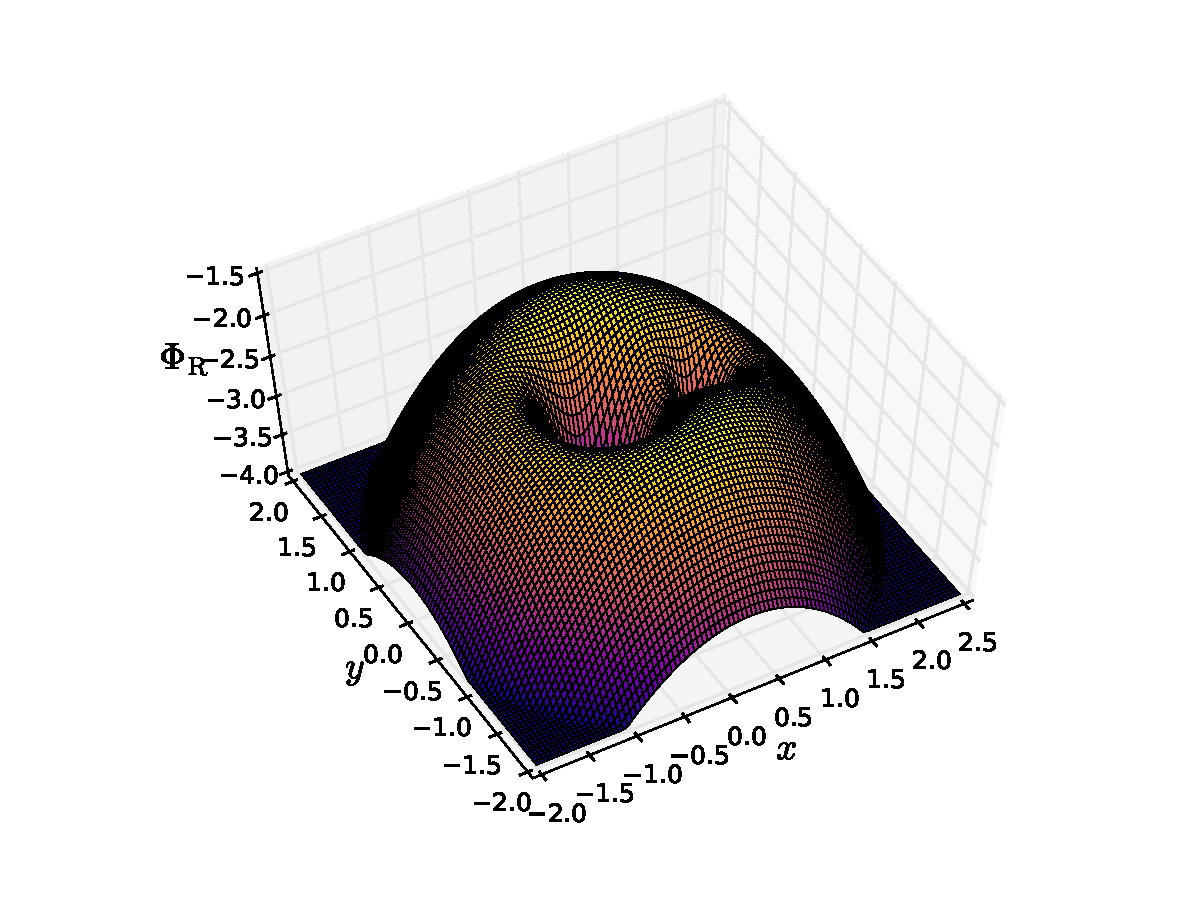
\includegraphics[width=7.5cm]{figs/astro/roche.pdf}
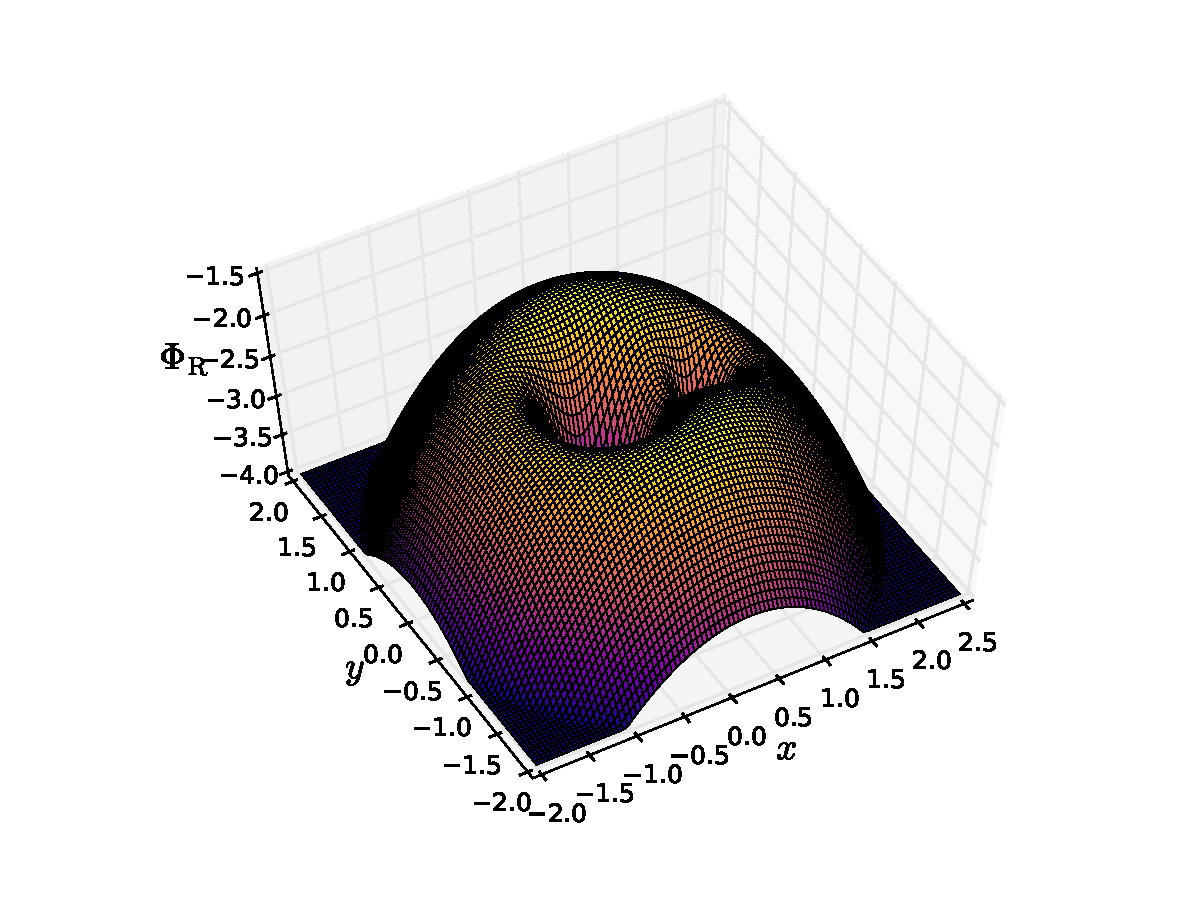
\includegraphics[width=7.5cm]{figs/astro/roche.pdf}
\caption{\label{fig:roche}
    Two-dimensional Roche potential $\Phi_{\mathrm{R}}(x,y)$ visualized for a binary systems with $M_1/M_2 = $ and $a = $.
}
\end{figure}

The effects originating from the gravitation and from the centrifugal forces are encapsulated in the so-called Roche potential, given as a function of radial vector $\vec{r}$ as\cite[see, e.g.,][]{PRP02, LL15}
\be
\Phi_{\mathrm{R}}(\vec{r}) = -\frac{G M_1}{|\vec{r} - \vec{r_1}|} -\frac{G M_2}{|\vec{r} - \vec{r_2}|} - \frac{1}{2} ( \vec{ \omega } \times \vec{v} )^2,
\ee
where the location of the stars are given with $\vec{r_1}$ and $\vec{r_2}$.
By studying the shape of the potential, we see that in between the stars, in the so-called $L_1$ point there exists a location where the countering gravitational forces from the two stars are balanced.
This can be though of as a physical nozzle in the system from which the less massive star will leak into the more massive star.
Such a mass transfer, also known as a Roche lobe overflow, will then occur if the companion star's radius exceeds the size of its own individual Roche lobe visualized in \fig{fig:roche}.
Typically such a thing can happen when the star evolves and expands at the end of its life cycle. 


\subsection{Accretion disks}
accretion disk: machine for slowly lowering material in the graviational potential and extracting energy
orbital kinetic energy to heat
Keplerian rotation law 
\be
\Omega_{\mathrm{K}}(R) = \left( \frac{G M }{R^3} \right)^{1/2}
\ee
implies differential rotation.
Viscous stress from shear viscosicty.

Reynolds number for the disk (inertia / viscous dissipation)
\be
\mathcal{R} \sim \frac{ v_{\phi}^2 / R }{\lambda \bar{v} v_{\phi} /R^2} = \frac{R v_{\phi}}{\lambda \bar{v}}
\ee
Molecular viscosity for $\lambda \sim \lambda_{\mathrm{D}}$ and $\bar{v} \sim c_{\mathrm{s}}$.
For typical accretion disk environment molecular $\mathcal{R} > 10^{14}$, i.e. highly turbulent.
Typical size of the turbulent eddies can not exceed the disk thickness $H$.
Velocity is most likely below sound speed $c_{\mathrm{s}}$ as otherwise turbulent motions would be thermalized by shocks from the supersonic motion.
Hence
\be
\nu = \alpha c_{\mathrm{s}} H
\ee
and we expect $\alpha \lesssim 1$. 
Reparameterizaton of our ignorance.
This is the $\alpha$-prescription by Shakura and Sunyaev.\cite{SS73}

\cite{Cho98}
Hydrodynamics of disks.




%Roche Lobe \cite{PRP02} \cite{LL15}
%LMXB \cite{TH06}

Hard and soft state \cite{HvdK89}
Alternates between these two states \cite{MDF14} \cite{DGK07}



\subsection{Between the disk and the star: boundary layers}

\be
\Omega(R) \approx \Omega_{\mathrm{K}}(R) = \left( \frac{G M}{R^3} \right)^{1/2}
\ee

Layer of thickness $b$ equals $\Omega(R + b) \approx \Omega_{\mathrm{K}}(R + b)$ that must slow down to $\Omega_{*}$.

Energy difference
\be
\dot{E} = \frac{1}{2} \Mdot R^2 (\Omega_{\mathrm{K}}^2 - \Omega_{*}^2) = 
\frac{1}{2} \Mdot \frac{GM}{R} \left[ 1 - \left(\frac{\Omega_*}{\Omega_{\mathrm{K}}} \right)^2 \right] 
\ee

Viscous torque $G_{\mathrm{T}} = \Mdot R^2 (\Omega_{\mathrm{K}} - \Omega_*)$
Hence,
\be
\dot{E} = \frac{1}{2} \frac{G M \Mdot}{R} \left( 1 - \frac{\Omega_*}{\Omega_{\mathrm{K}}} \right)^2
\ee


\section{X-ray bursts}
\subsection{Unstable thermonuclear burning on top of neutron stars}

\subsection{Constraining the size of bursting source}



